\documentclass[11pt]{thyv}

\usepackage[utf8]{inputenc}

    \definecolor{thyFirst}{RGB}{132,70,132}
    \definecolor{thySecond}{RGB}{70,70,132}
    \definecolor{thyThird}{RGB}{170,60,60}
    \definecolor{thyGrey}{RGB}{100,100,100}

\begin{document}
	\begin{textblock}{5}(0.5, 0)
		\begin{center}
			\begin{tikzpicture}[x=\imagescale,y=-\imagescale]
				\clip (300, 300) circle (300);
				\draw[line width=2pt] (300, 300) circle (300);
				\node[anchor=north west, inner sep=0pt, outer sep=0pt] at (0,0) {
					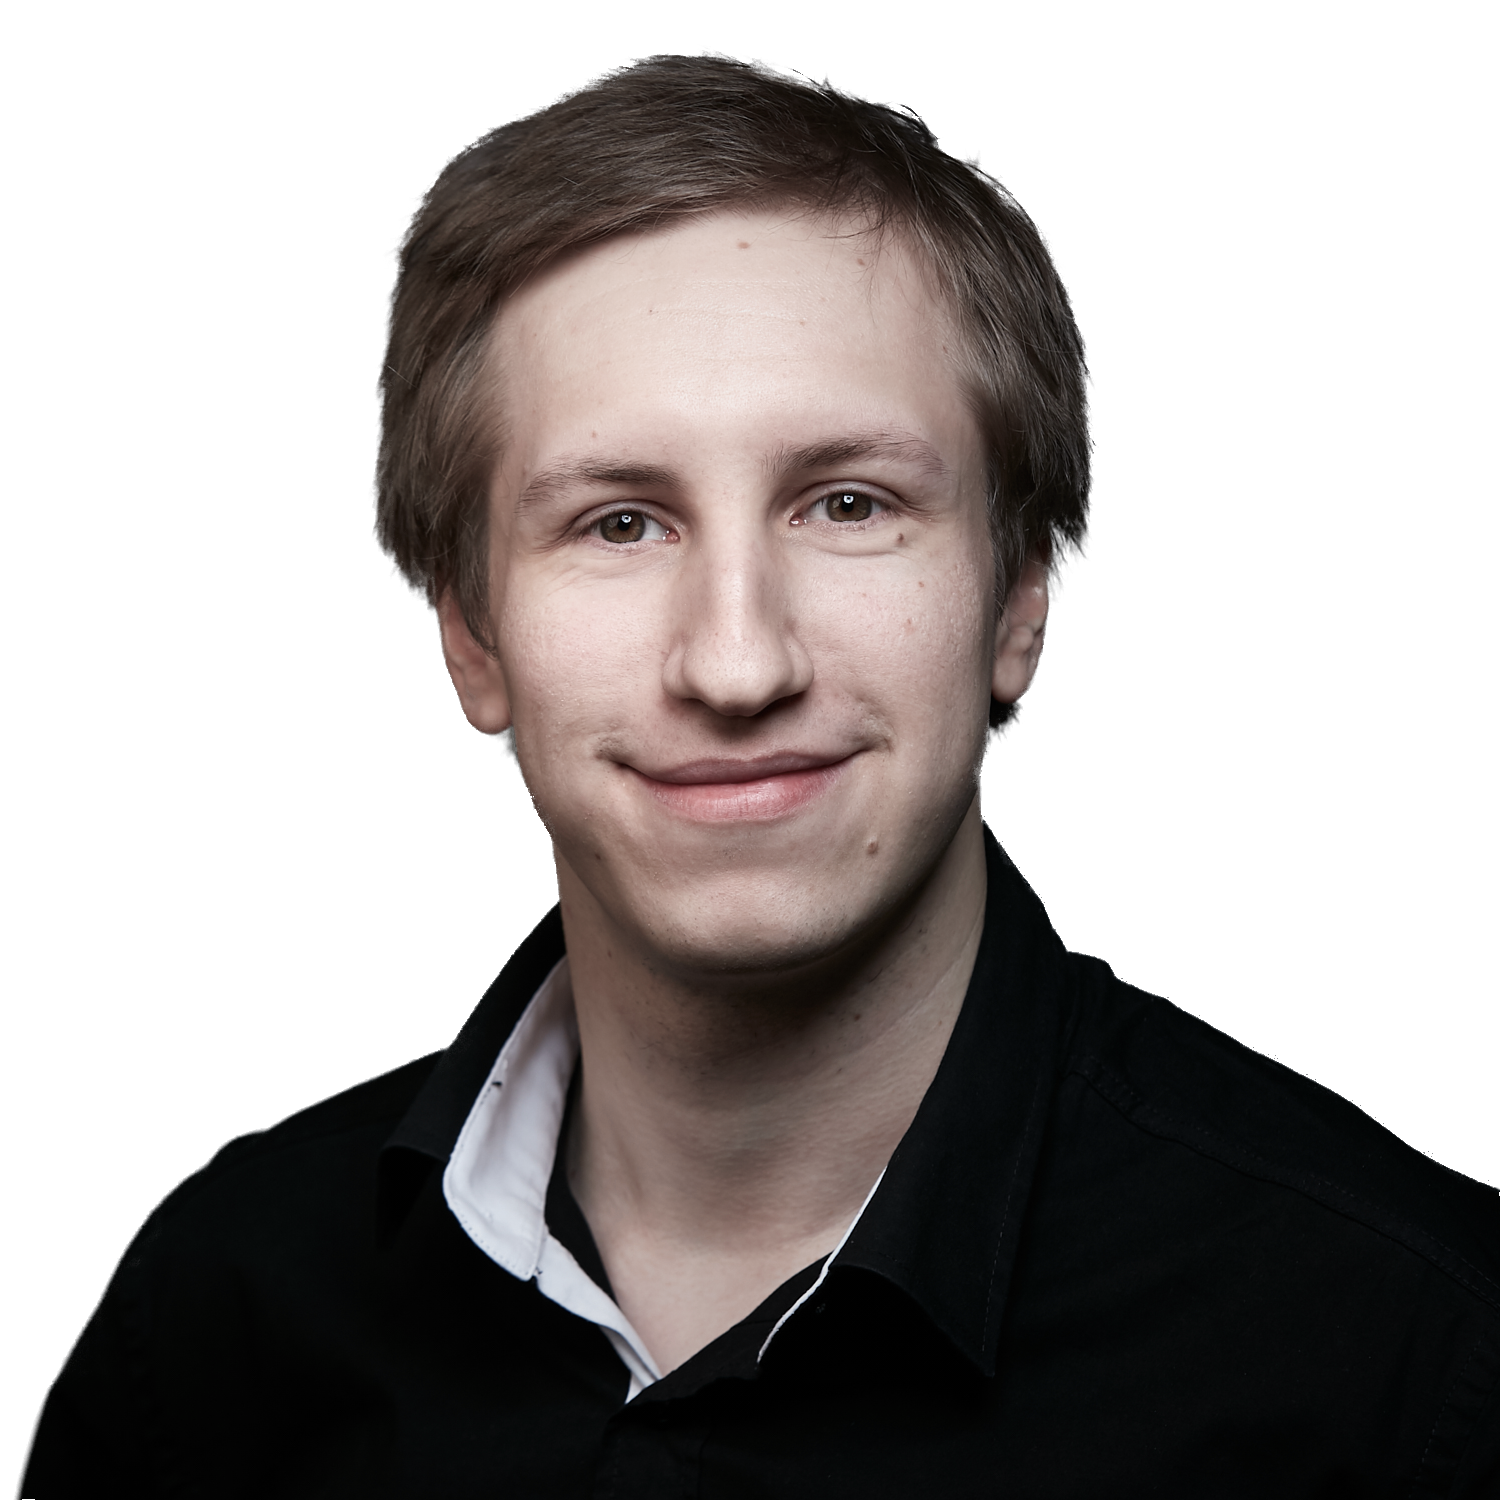
\includegraphics[width=\imagewidth]{max0.6.png}
				};
			\end{tikzpicture}
		\end{center}
		{\Large\textbf{\texttt{Max-Jonathan Luckow}}}\\
		Computer Science Student\\

		\begin{thyV}{2010}{2024}{22.1}{0.6\linewidth}
			\thyVent{high-school\\ diploma} 					{6/2010}
			\thyVent{Publication} 								{1/2020}
			\thyVent{B.Sc.Thesis} 							{3/2017}
			\thyVent{M.Sc.Thesis} 							{3/2023}

			\thyVentEdu{Energy and Process 	\\Engineering} 		{4/2011}{9/2013} 	{}
			\thyVentEdu{Bachelor of Science \\Computer Science} {10/2013}{3/2017} 	{16.625/2014}
			\thyVentEdu{Master of Science 	\\Computer Science} {4/2017}{3/2023} 	{7.25/2020}

			\thyVentWork{Technical Accountant} 				{9/2020}{4/2022} 	{}
			\thyVentWork{Web Developer} 						{3/2018}{4/2018} 	{}
			\thyVentWork{Technical Specialist} 					{6/2017}{11/2017} 	{9.25/2017}
			\thyVentWork{Self-employed} 						{1/2014}{5/2017} 	{22.875/2014}

			\thyVentWork{Assistant in \\ surgical ward} 		{8/2010}{1/2011} 	{12/2010}
		\end{thyV}
	\end{textblock}
	\begin{mdframed}
		\begin{minipage}[t]{0.50\textwidth}
			\vspace{-\baselineskip}
			\icon{StarOfLife}{12}{30. December 1990}\\
			\icon{Phone}{12}{+49 163 222 99 64}
		\end{minipage}
		\begin{minipage}[t]{0.50\textwidth} 
			\vspace{-\baselineskip}
			\icon{Github}{12}{\href{https://github.com/Carlisle96}{github.com/Carlisle96}}\\
			\icon{At}{12}{\href{mailto:max@luckow.ch}{max@luckow.ch}}
		\end{minipage}

		\thyVsection{Publication}{thyThird}
			M. J. Luckow and T. Fluschnik. \textbf{``\href{https://doi.org/10.1016/j.ipl.2019.105913}{On the Computational Complexity of Length- and Neighborhood-Constrained Path Problems}''}. In: \textit{Information Processing Letters.} Vol. 156 (2020). \texttt{\doi{10.1016/j.ipl.2019.105913}}\hfill \textcolor{thyGrey}{1/2020}

		\thyVsection{Work Experience}{thySecond}
			\thyntry{Technical Acountant}{Agilo-Services GmbH}{9/2020 -- present}
			{Project analysis, optimization, automation and supervision of the accounting system}
			{Datev Uno \slashsep Haskell}

			\thyntry{Web Developer}{Trado GmbH}{3/2018 -- 4/2018}
			{Development of the core backend and enterprise administrative software solution}
			{Javascript \slashsep Node.js \slashsep Vue.js \slashsep SQL}

			\thyntry{Technical Specialist}{Envion AG}{6/2017 -- 11/2017}
					{Strategy planning, devolopment of the first mining prototype and supervision of the production of the first large scale mining operation with \$100 million market value}
			    	{Linux \slashsep Solidity}

			\thyntrySmall{Self-employed}{}{1/2014 -- present}
			{IT administration, development and project support}

			%\thyntrySmall{Assistant in surgical ward}{Hospital Waldfriede Berlin}{08/2010 -- 01/2011}
			%{Community service}

		\thyVsection{Education}{thyFirst}
			\thyntry{Master of Science. Computer Science}{Technical University of Berlin}{4/2017 -- \textit{3/2023}}{Specialisation in cognitive systems}{Java \slashsep Python \slashsep Solidity}

			\thyntry{Bachelor of Science. Computer Science}{Technical University of Berlin}{10/2013 -- 3/2017}{Area of study in foundations of computing with a thesis on algorithms and complexity}{Java \slashsep C/\CplusplusSpace \slashsep Python \slashsep SQL \slashsep Latex}{}

			\thyntrySmall{Energy and Process Engineering}{Technical University of Berlin}{4/2011 -- 9/2013}{\texttt{Fortran \slashsep Latex}}

			%\thyntrySmall{High-school diploma}{Arndt Gynasium Dahlem}{8/2003 -- 6/2010}{}

		\begin{minipage}[t]{0.45\textwidth}
			\vspace{-0.5\baselineskip}
			\thyVsection{Interests}{thyBlack}
			\vspace*{-12pt}
			\hspace{-12pt}\thyChart
		\end{minipage}
		\begin{minipage}[t]{0.55\textwidth}
			\vspace{-0.5\baselineskip}
			\thyVsection{Technical Expertise}{thyBlack}
			\begin{barchart}{5}
				\baritem{Linux}{70}
				\baritem{LaTeX}{100}
				\baritem{C/\Cplusplus}{50}
				\baritem{Java}{80}
				\baritem{Python}{60}
				\baritem{Javascript}{40}
				\baritem{SQL}{20}
				\baritem{Solidity}{30}
				\baritem{Haskell}{10}
			\end{barchart}
		\end{minipage}
		\vspace*{-20pt}

		\thyVsection{Language}{thyBlack}
			German: Native speaker \\
			English: Fluent \\
			Latin: Latinum
		\begin{textblock}{5}(17.5, 27.5)
			
\includegraphics[width=3cm]{signature2.png}
		\end{textblock}
	\end{mdframed}
\end{document}